\documentclass[10pt,landscape,a4paper]{article}
\usepackage[utf8]{inputenc}
\usepackage[ngerman]{babel}
\usepackage[T1]{fontenc}
%\usepackage[LY1,T1]{fontenc}
%\usepackage{frutigernext}
%\usepackage[lf,minionint]{MinionPro}
\usepackage{tikz}
\usetikzlibrary{shapes,positioning,arrows,fit,calc,graphs,graphs.standard}
\usepackage[nosf]{kpfonts}
\usepackage[t1]{sourcesanspro}
\usepackage{multicol}
\usepackage{wrapfig}
\usepackage[top=0mm,bottom=1mm,left=0mm,right=1mm]{geometry}
\usepackage[framemethod=tikz]{mdframed}
\usepackage{microtype}
\usepackage{pdfpages}
\usepackage{graphics}
\usepackage{mathtools}

\let\bar\overline

\definecolor{myblue}{cmyk}{1,.72,0,.38}

\def\firstcircle{(0,0) circle (1.5cm)}
\def\secondcircle{(0:2cm) circle (1.5cm)}

\colorlet{circle edge}{myblue}
\colorlet{circle area}{myblue!5}

\tikzset{filled/.style={fill=circle area, draw=circle edge, thick},
    outline/.style={draw=circle edge, thick}}
    
\pgfdeclarelayer{background}
\pgfsetlayers{background,main}

\everymath\expandafter{\the\everymath \color{myblue}}
\everydisplay\expandafter{\the\everydisplay \color{myblue}}

\renewcommand{\baselinestretch}{.8}
\pagestyle{empty}

\global\mdfdefinestyle{header}{%
linecolor=gray,linewidth=1pt,%
leftmargin=0mm,rightmargin=0mm,skipbelow=0mm,skipabove=0mm,
}

\newcommand{\header}{
\begin{mdframed}[style=header]
\footnotesize
\sffamily
Hilfszettel zur Klausur\\
von \textbf{JD}.,~Seite~\thepage~von~2
\end{mdframed}
}

\makeatletter % Author: https://tex.stackexchange.com/questions/218587/how-to-set-one-header-for-each-page-using-multicols
\renewcommand{\section}{\@startsection{section}{1}{0mm}%
                                {.2ex}%
                                {.2ex}%x
                                {\color{myblue}\sffamily\small\bfseries}}
\renewcommand{\subsection}{\@startsection{subsection}{1}{0mm}%
                                {.2ex}%
                                {.2ex}%x
                                {\sffamily\bfseries}}



\def\multi@column@out{%
   \ifnum\outputpenalty <-\@M
   \speci@ls \else
   \ifvoid\colbreak@box\else
     \mult@info\@ne{Re-adding forced
               break(s) for splitting}%
     \setbox\@cclv\vbox{%
        \unvbox\colbreak@box
        \penalty-\@Mv\unvbox\@cclv}%
   \fi
   \splittopskip\topskip
   \splitmaxdepth\maxdepth
   \dimen@\@colroom
   \divide\skip\footins\col@number
   \ifvoid\footins \else
      \leave@mult@footins
   \fi
   \let\ifshr@kingsaved\ifshr@king
   \ifvbox \@kludgeins
     \advance \dimen@ -\ht\@kludgeins
     \ifdim \wd\@kludgeins>\z@
        \shr@nkingtrue
     \fi
   \fi
   \process@cols\mult@gfirstbox{%
%%%%% START CHANGE
\ifnum\count@=\numexpr\mult@rightbox+2\relax
          \setbox\count@\vsplit\@cclv to \dimexpr \dimen@-1cm\relax
\setbox\count@\vbox to \dimen@{\vbox to 1cm{\header}\unvbox\count@\vss}%
\else
      \setbox\count@\vsplit\@cclv to \dimen@
\fi
%%%%% END CHANGE
            \set@keptmarks
            \setbox\count@
                 \vbox to\dimen@
                  {\unvbox\count@
                   \remove@discardable@items
                   \ifshr@nking\vfill\fi}%
           }%
   \setbox\mult@rightbox
       \vsplit\@cclv to\dimen@
   \set@keptmarks
   \setbox\mult@rightbox\vbox to\dimen@
          {\unvbox\mult@rightbox
           \remove@discardable@items
           \ifshr@nking\vfill\fi}%
   \let\ifshr@king\ifshr@kingsaved
   \ifvoid\@cclv \else
       \unvbox\@cclv
       \ifnum\outputpenalty=\@M
       \else
          \penalty\outputpenalty
       \fi
       \ifvoid\footins\else
         \PackageWarning{multicol}%
          {I moved some lines to
           the next page.\MessageBreak
           Footnotes on page
           \thepage\space might be wrong}%
       \fi
       \ifnum \c@tracingmulticols>\thr@@
                    \hrule\allowbreak \fi
   \fi
   \ifx\@empty\kept@firstmark
      \let\firstmark\kept@topmark
      \let\botmark\kept@topmark
   \else
      \let\firstmark\kept@firstmark
      \let\botmark\kept@botmark
   \fi
   \let\topmark\kept@topmark
   \mult@info\tw@
        {Use kept top mark:\MessageBreak
          \meaning\kept@topmark
         \MessageBreak
         Use kept first mark:\MessageBreak
          \meaning\kept@firstmark
        \MessageBreak
         Use kept bot mark:\MessageBreak
          \meaning\kept@botmark
        \MessageBreak
         Produce first mark:\MessageBreak
          \meaning\firstmark
        \MessageBreak
        Produce bot mark:\MessageBreak
          \meaning\botmark
         \@gobbletwo}%
   \setbox\@cclv\vbox{\unvbox\partial@page
                      \page@sofar}%
   \@makecol\@outputpage
     \global\let\kept@topmark\botmark
     \global\let\kept@firstmark\@empty
     \global\let\kept@botmark\@empty
     \mult@info\tw@
        {(Re)Init top mark:\MessageBreak
         \meaning\kept@topmark
         \@gobbletwo}%
   \global\@colroom\@colht
   \global \@mparbottom \z@
   \process@deferreds
   \@whilesw\if@fcolmade\fi{\@outputpage
      \global\@colroom\@colht
      \process@deferreds}%
   \mult@info\@ne
     {Colroom:\MessageBreak
      \the\@colht\space
              after float space removed
              = \the\@colroom \@gobble}%
    \set@mult@vsize \global
  \fi}

\makeatother
\setlength{\parindent}{0pt}

\begin{document}
%\footnotesize
\small
\begin{multicols*}{5}
%There must be Content because error: pdf does not look lke a valid PDF document. Either the file is corrupt or it is in the process of creation. Retrying every two seconds
\section{BeschreibendeStatistik}
  \subsection{Begriffe}
    \subsubsection{Beschreibende/Deskriptive Statistik}
    Beobachtete Daten werden durch geeignete statistische Kennzahlen charakterisiert und durch geeignete Grafiken anschaulich gemacht.
    \subsubsection{Schließende/Induktive Statistik}
    Aus beobachtete Daten werden Schlüsse gezogen und diese im Rahmen vorgegebener Modelle der Wahrscheinlichkeitstheorie bewertet.
    \subsubsection{Grundgesamtheit}
    $\Omega$: Grundgesamtheit
    $\omega$:Element oder Objekt der Grundgesamtheit
    diskret(<30 Ausprägungen), stetig($\geq$30 Ausprägungen), univariat(p=1), mulivariat(p>1); Diskrete Merkmale haben eine abzählbare Anzahl möglicher Ausprägungen. Stetige Merkmale habne eine nicht abzählbare (=überabzählbar) Anzahl möglicher Ausprägungen.
  \subsection{Lagemaße}
    \subsubsection{Modalwerte $x_{mod}$}
    Am häufigsten auftretende Ausprägungen (insbesondere bei \textbf{qualitativen} Merkmalen)
\subsubsection{Mittelwert, quantitativ}
    R:$mean(x)$\\
    Schwerpunkt der Daten.\textbf{Empfindlich}gegemüber Ausreißern.
    $\overline{X} = \frac{1}{n} \sum_{i=1}^{n} x_{i}$
    \subsection{Median, quantitativ}
    R:$median(x)$\\
    Liegt in der Mitt der sortierten Daten $x_{i}$. \textbf{Unempfindlich} gegenüber Ausreißern.
    \begin{equation}
      x_{0.5} =
        \begin{cases}
        	x_{\frac{n+1}{2} \text{, falls n ungerade}}\\
        	\frac{1}{2}(x_{\frac{n}{2}} + x_{\frac{n}{2}+1}) \text{, falls n gerade}
        \end{cases}
    \end{equation}
  \subsection{Streuungsmaße}
    \subsubsection{Spannweite}
    max $x_{i}$ - min $x_{i}$
    \subsubsection{Stichprobenvarianz $s^2$}
    R:$var(x)$\\
    \textbf{Verschiebungssatz:}\\
      $s^2 = \frac{1}{n-1} \sum_{i=1}^{n}(x_{i} - \overline{x}^2) = \frac{1}{n-1} (\sum_{i=1}^{n} x_{i}^2 - n\overline{x}^2)$
      Gemittelte Summe der quadratischen Abweichung vom Mittelwert
      \subsubsection{Stichproben-\\standardabweichung}
      R:$sd(x)$\\
      $s=\sqrt{s}$
      Streuungsmaß mit gleicher Einheit wie beobachteten Daten $x_{i}$.$ \overline{x}$ minimiert die "quadratische Verlustfunktion" oder die Varianz gibt das Minimum der Fehlerquadrate an.
      \subsection{p-Quantile}
      R:$quantile(x,p)$. Teilt die \textbf{sortierten} Daten $x_{i}$ ca. im Verhältnis p: (1-p) d.h. $\hat{F}(x_{p)} \approx p$; 
      $\hat{F} \hat{=} $ kummul. rel. Häufigkeit; 
      1. Quartil = 0.25-Quantil; 
      Median = 0.5-Quantil; 
      3. Quartil = 0.75-Quartil; 
      \begin{equation}
      	x_{p}
        \begin{cases}
          x_{floor(np) +1} , np \in \mathbb{N}\\
          \frac{1}{2} (x_{np} + x_{np+1}, np \notin \mathbb{N})\\
        \end{cases}
      \end{equation}
      \subsection{Interquartilsabstand I}
      $I = x_{0.75} - x_{0.25}$. Ist ein weiterer Streuungsparameter.
      \subsection{Chebyshev}
      $\frac{N(S_{k})}{n} > 1-\frac{1}{k^2}$, für alle k $\geq$ 1
      $\overline{x}$ der Durchschnitt, s > 0 die Stichproben-Standardabweichung von Beobachtungswerten $x_{1}, ..., x_{n}$. Sei $S_{k} = \{i, 1 \leq i \leq n: |x_{i} - \overline{x}| < k \cdot s\}$; Für eine beliebige Zahl k $\geq$ 1 liegen mehr als $100 \cdot (1-\frac{1}{k^2})$ Prozent der Daten im Intervall von $\overline{x} - ks$ bis $ \overline{x} + ks$. \textbf{Speziell:}Für k = 2 liegen mehr als 75\% der Daten im 2s-Bereich um $\overline{x}$. Für k=3 liegen mehr als 89\% der Daten im 3s-Bereich um $\overline{x}$. \textbf{Komplement Formulierung:} $\overline{S}_{k} = \{i | |x_{i}-\overline{x}| \geq k \cdot s\}$; 
      $\frac{N(\overline{S}_{k})}{n} \leq \frac{1}{k^2}$; Die Ungleichheit lifert nur eine \textbf{sehr grobe Abschätzung}, ist aber unabhängig von der Verteilung der Daten. \textbf{Empirische Regeln} 68\% der Daten im Bereich um $\overline{x} \pm s$. 95\% um $\overline{x} \pm 2s$. 99.7\% um $\overline{x} \pm3s$.
      \subsection{Korrelation}
      Grafische Zusammenhang zwischen multivariaten Daten x und y durch ein Streudiagramm. Kennzahlen zur Untersuchung des Zusammenhangs:
      \subsubsection{Empirische Kovarianz}
      R:$cov(x,y)$;
      $s_{xy} = \frac{1}{n-1}\sum_{i=1}^{n}(x_{i}-\overline{x})(y_{i}-\overline{y})=\frac{1}{n-1}(\sum_{i=1}^{n}(x_{i}y_{i})- n\overline{x}\overline{y})$; 
      $ S_{xy} > 0 $ steigend; 
      $ S_{xy} < 0 $ fallend; 
      \subsubsection{Empir. Korrelk.koeff. r}
      R:$cor(x,y)$;
      $r = \frac{s_{xy}}{s_{x}s_{y}}$; Näherungsweise lin. Zusammenhang zw. x und y, falls |r| $\approx$1;
      \textbf{Bemerkung}: -Der Korrelationskoeffizient kann nur einen statistischen Zusammenhang beschreiben, keinen Kausalen; -Den Korrelationskoeffizient immer im Zusammenhang mit den Streudiagramm sehen (Anscombe-Quartett).
      \subsubsection{Regressionsgerade y}
      $y = mx + t$ mit $m=r \cdot \frac{s_{y}}{s_{x}}$ und $ t=\overline{y} -m \cdot \overline{x}$;
      Für den Bereich $|\pm$0,7|$ bis $ bis $\pm 1   \Rightarrow $ linearer Zusammenhang.
\section{Wahrscheinlichkeitsrechnung}
  \subsection{Begriffe}
  \textbf{Ergebnisraum} $\Omega$: Menge aller möglichen Ergebnisse eines Experiments\\
  \textbf{Elementarereignis} $\omega \in \Omega$: einzelnes Element von $\Omega$\\
  \textbf{Ereignis}$E \subseteq \Omega$: beliebige Teilmenge des Ergebnisraums $\Omega$ heißt sicheres Ereignis, $\emptyset$ heißt unmögliches Ereignis\\
  \textbf{Vereinigung} $E \cup F$: Ereignis E oder Ereignis F treten ein. $\bigcup_{i=1}^{n} E_{i}$: mindestens ein Ereignis $E_{i} $tritt ein.\\
  \textbf{Schnitt} $E \cap F$: Ereignis E und Ereignis F treten ein.\\
  $\bigcap_{i=1}^{n} E_{i}$ alle Ereignisse $E_{i}$ treten ein.
  \textbf{Gegenereignis} $\overline{E} = \Omega /\ E$: Ereignis E tritt nicht ein (Komplement von E)\\
  \textbf{Disjunkte Ereignisse}E  und F: $E \cap F = \emptyset$
  \subsection{De Morgan'schen Regeln}
  $\overline{E_{1} \cup E_{2}} = \overline{E}_{1} \cap \overline{E}_{2}$\\
  $ \overline{E_{1} \cap E_{2}} = \overline{E}_{1} \cup \overline{E}_{2}$
  \subsection{Wahrscheinlichkeit}
  $0 \le P(E) \le 1$; P($\Omega$) = 1;\\
  P($\bigcup_{i=1}^{\infty}) = \sum_{i=1}^{\infty}$ P($E_{i}$), falls $E_{i} \cap E_{j} = \emptyset$ für $i \neq j$\\
    \subsection{Satz 2.1}
    P($\overline{E}$) = 1 -P(E)\\
    P($E \cup F$) = P(E)+ P(F) - P($E \cap F$)
  \textbf(Übungsaufgabe!!! Ergänzen)\\
  \subsection{Laplace-Experiment}
  Zufallsexperimente mit n gleich wahrscheinlichen Elementarereignissen. Dann berechnet sich die Wahrscheinlichkeit P(E) für $E \subseteq \Omega$ aus:\\
  P(E) =$\frac{\text{Anzahl der für E günstigen Ereignisse}}{\text{Anzahl der möglichen Ereignisse}} = \frac{\text{Mächtigkeit von E}}{\text{Mächtigkeit von } \Omega} = \frac{|E|}{n}$
%  \subsection{Kombinatorik}
%  \subsubsection{Allgmeines Zählprinzip}
%  Anzahl der Möglihckeiten für ein k-stufiges Zufallsexperiment mit $n_{i}$ Varianten im i-ten Schritt:
%  $n_{1} \cdot n_{2} \cdot \text{...} \cdot n_{k}$
%  \subsubsection{Permutationen}
%  Anzahl einer n-elementigen Menge n-maliges Ziehen ohne Zurücklgen mit Beachtung der Reihenfolge: \textbf{n unterscheidbare Elemente}: $n! = n \cdot(n-1) textbf{...} 2 \cdot 1$
%  \textbf{k Klassen mit je $n_{i}$ nicht unterscheidbaren Elementen} $n = sum_{k }^{i=1} n_{i}$:
%  $\frac{n!}{n_{1}! \cdot n_{2}!\cdot \text{...}n_{k}! }$
%  \subsubsection{Anzahl k-elementigen Teilmengen einer n-elementigen Menge k-maliges Ziehen aus einer n-elementigen Menge}
%  ohne Zurücklegen = $k\le n$.\\
%  mit Zurücklegen = $ k > n$ möglich.\\
%  \textbf{mit Beachtung der Reihenfolge, ohne Zurücklegen}: $\frac{n!}{(n-k)!}$\\
%  \textbf{ohne Beachtung  der Reihenfolge, ohne Zurücklegen}: $\binom{n}{k} = \frac{n!}{(n-k)! k!}$\\
%  \textbf{mit Beachtung der Reihenfolge, mit Zurücklegen}: $n^k$\\
%  \textbf{ohne Beachtung der Reihenfolge, mit Zurücklegen} $\binom{n+k-1}{k}$
  \subsection{Bedingte Wahrscheinlichkeit}
  $P(E|F) = P_{F}(E) = \frac{|E \cap F| }{|F|} = \frac{P(E\cap F)}{P(F)}$
  \subsection{Satz 2.2}
  $P(E \cap F) = P(E|F) \cdot P(F)$\\
  $P(E \cap F) = P(F|E) \cdot P(E)$\\
  	
\includegraphics[scale=0.2]{./pic/BedingteWahrscheinlichkeit.png}
  	\subsection{Satz der totalen Wahrscheinlichkeit}
  	Sei $\Omega = \bigcup_{i=1}^{n} E_{i}$ mit $E_{i} \cap E_{j} =  \varnothing$ für $i \ne j$ d.h. die Ereignisse bilde eine disjunkte Zerlegung bzw. eine Partition von $\Omega$. Somit gilt:\\
  	$P(F) = \sum_{i=1}^{n} P(F \cap E_{i}) = \sum_{i=1}^{n} P(F|E_{i}) \cdot P(E_{i})$\\
  	Summe der Äste des Wahrscheinlichkeitsbaums zu allen Schnitten $F \cap E_{i}$
  	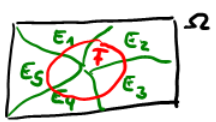
\includegraphics[scale=0.25]{./pic/SatzTotalerWahrscheinlichkeit.png}
  	\subsection{Vierfeldertafel}
  	$ P(F) = P(F \cap E ) + P(F \cap \overline{E}) $\\
  	$ P(\overline {F}) = P(\overline{F} \cap E) + P(\overline{F} \cap E) $\\
  	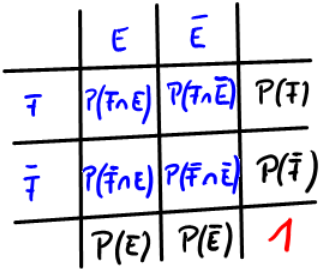
\includegraphics[scale=0.25]{./pic/Vierfeldertafel}
  	\textbf{Satz 2.2 oben: }
  	$ P(E \cap F)  =  P(E) \cdot P(F|E) = P(F) \cdot P(E|F) $
  	\textbf{Tafel}
  	$ = P(F) - P(F \cap \overline{E}) $
  	$ = P(E) - P(\overline{F} \cap E) $; 
  $ P(\overline{F} | E) = 1 - P(F | E) $
  \subsection{Formel von Bayes}
  Hilfreich, wenn man man $P( F | E_{i} )$ kennt, aber nicht $P(E_{k}|F)$
  \textbf{Satz 2.4}
  $P(E_{k} | F) = \frac{ P(F | E_{k}) \cdot P(E_{k})}{ \underbrace{\sum_{i=1}^{n}P(F|E_{i}) \cdot P(E_{i})}}$\\
\textbf{Nur Nenner!}P(F) aus dem Satz der totalen Wahrscheinlichkeit.
  \subsection{Stochastische Unabhängigkeit}
  \textbf{Übung}
  Die Ereignisse E und F heißen (stochastisch) unabhängig, wenn die Information über das Eintreten des einen Ereignisses die Wahrscheinlichkeit für das Eintreten des anderen Ereignisses nicht ändert, d.h. falls\\
  $\underbrace{P(E|F)}= P(E)  \text{ or }   P(E\cap F) = P(E) \cdot P(F)$\\
  $= \frac{P(E \cap F)}{P(F)}$\\
  \textbf{Es gilt}
  Falls die Ereignisse E, F unabhängig sind, dann sind auch: 
  $\circ  E, \overline{F}$;  
  $\circ  \overline{E} , F$;  
  $\circ \overline{E}, \overline{F}$ unabhängig\\
  \textbf{Bemerkung}\\
  	$ \circ $ Stochastische Unabhängigkeit bedeutet nicht notwendigerweise eine kausale Abhängigkeit; 
  	$ \circ $ Veranschaulichung mit Venn Diagramm
  	  \includegraphics[scale=0.23]{./pic/StochastischeUnabhängigkeit.png}
  	  \includegraphics[scale=0.23]{./pic/StochastischeAbhängigkeit.png}\\
  	$\circ$ $A, B \ne \varnothing$ und $A \cap B  = \varnothing$\\
  	$P(A\cap B) \stackrel{?}{=} P(A) \cdot P(B)$\\
  	$ \varnothing \ne P(A) \cdot P(B)$ da P(A) > 0 und P(B)> 0\\
  	=> A, B stochastisch abhängig
\section{Zufallsvariable}
Abbildung des \textbf{abstrakte} Ergebnisraums $\Omega$ auf $\mathbb{R}$.
Eine Abbildung $X: \Omega \rightarrow \mathbb{R}$, $\omega \mapsto X(\omega)$ = heißt Zufallsvariable (ZV). x $\in$ R. heißt Realisation der ZV X.
  \begin{itemize}
    \item Diskrete ZV: $X(\Omega) = {x_{1}, ..., x_{2}} (n \in \mathbb{N})$; z.B. X = \dq Augensumme beim Würfeln \dq
    \item Stetige ZV: $X(\Omega) \subseteq \mathbb{R}$; \dq z.B. Körpergröße eines Menschen\dq
  \end{itemize}
\subsection{Verteilungsfunktion-allg.}
Die Wahrscheinlichkeit P(B) für ein Ereignis B in $\mathbb{R}$ wird zurückgefürht auf die Wahrscheinlichkeit der entsprechenden Ereignisse in $\Omega$. Für jedes $X \in \mathbb{R}$  ist die Verteilungsfunktion F: $\mathbb{R} \rightarrow [0,1]$ einer ZV X definiert durch:\\
	F(x) = P(X $\leq$ x)
\begin{itemize}
	\item $0 \leq F(x) \leq 1$
	\item $\lim\limits_{x\to-\infty} F(X)= 0 \, \lim\limits_{x\to\infty} F(x) = 1$
	\item monoton wachsend
	\item $P(X > x) = 1 - F(x)$
	\item $P(a < X \leq b) = F(b) - F(a)$
\end{itemize}
\subsection{Diskrete ZVs}
Für eine diskrete ZV X mit $X(\Omega) = {x_{1}, ..., x_{n}}$ ( n endlich oder abzählbar unendlich) ist die Wahrscheinlichkeitsfunktion definiert durch:\\
\begin{equation}
p(x) =
\begin{cases}
	P(X = x_{i}), \text{falls } x_{i} \in X(\Omega )\\
	0, sonst\\
\end{cases}
\end{equation}
\textbf{Es gilt:}
\begin{itemize}
	\item $F(x) = (P(X \leq x) = \sum_{x_{i}\leq x} p(x_{i})$
	\item F(x) ist eine rechtseitig stetige \textbf{Treppenfunktion} mit \textbf{Sprüngen} bei der Realisation von $x_{i}$.
\end{itemize}
\subsection{Stegite ZVs}
Stetige ZV X ist die Wahrscheinlichkeitsdichte f $ f : \mathbb{R} \rightarrow [0,\infty[$ definiert durch\\
$P(a < X < b) = \int_{a}^{b} f(x) dx$\\
\textbf{Es gilt:}
\begin{itemize}
	\item $F(x) = P(X \leq x) = \int_{-\infty}^{x} f(t) dt$ und $F'(x) = f(x)$
	\item F(x) ist stetig \& $P(a < X \leq b) = P(a \leq X \leq b)$ wegen $P(X = a) = 0$
\end{itemize}
\subsection{Verteilungsfunktion}
$\int_{\textbf{Untergrenze}}^{x}$ Es wird normal mit - Integriert.
\subsection{Zusammenfassung}
\subsubsection{Diskrete ZV}
\begin{itemize}
	\item Wahrscheinlichkeitsverteilung p(x) $\sum_{i}^{n} p(x_{i}) = 1 x_{i}$ ist Realisation der ZV.
	\item Verteilungsfunktion F(x) ist rechtsseitig  stetige \textbf{Treppenfunktion}. \textbf{Sprunghöhen:}$P(X = x_{i}) = F(x_{i}) - \lim\limits_{x \to x_{i}-} \ne 0$
	\item $P(a < X \le b) = F(b)- F(a) \ne P(a \le X \le b)$
\end{itemize}
\subsubsection{Stetige ZV}
\begin{itemize}
	\item Dichtefunktion fx $\int_{-\infty}^{\infty} f(x) dx = 1$
	\item Verteilungsfunktion $F(x)$ ist stetig mit $F'(x) = f(x); P(X = x_{i}) = 0$
	\item $P(a < X \leq b ) = F(b) - F(a) = P( a \leq X \leq b) = F(a \leq X < b) = P(a < X < b)$
\end{itemize}
\subsection{Erwartungswert}
Der Erwartungswert $E[X] = µ$ einer ZV X ist der \textbf{Schwerpunkt} ihrer Verteilung \underline{or} der durchschnittliche zu erwartende Wert der ZV.
\begin{itemize}
  \item diskrete ZV: $E[X] = \sum_{i=1}^{n} x_{i} \cdot p(x_{i})$
  \item stetige ZV: $E[X] = \int_{-\infty}^{\infty} x \cdot f(x) dx$
\end{itemize}
ZV ist konstant. E[X] verhält sich linear. Eigenschaften von $E[X]$:
\begin{itemize}
  \item $E[b] = b$
  \item $E[aX + b] = aE[X] + b$
  \item $E[\underbrace{X_{i} + ... + X_{n}}] = \sum_{i=1}^{n} E[X_{i}]$
  \item $\sum_{i=1}^{n} x_{i}$
\end{itemize}
\subsubsection{Satz 3.1}
Sei Y = g(X) eine Funktion der ZV X. Dann gilt:
\begin{itemize}
  \item für diskrete ZV:$E[g(X)] = \sum_{i=1}^{n} g(x) \cdot p(x_ {i})$
  \item für stetige ZV: $E[g(X)] = \int_{-\infty}^{infty} g(x) \cdot f(x) dx$. Das vertauschen von E und g nur bei \textbf{linearen} Funktionen möglich. $\Rightarrow$ g(E[X])
\end{itemize}
\subsection{Varianz}
Die Varianz einer ZV X mit µ ist ein quadratisches Streungsmaß. $\sigma^2 = Var[X] = E[\underbrace{(X - µ)^2}] \stackrel{\text{falls x stetig}}{=} \int_{-\infty}^{\infty} (x-\mu)^2 \cdot f(x)$\\
g(X)\\
Die Standardabweichung $\sigma = \sqrt{Var[X]}$ hat im Gegensatz zur Varianz die gleiche Dimension von die ZV X.
\begin{itemize}
  \item $Var[b] = 0$
  \item $Var[aX + b] = a^2 Var[X]$
\end{itemize}
\subsubsection{Satz 3.2}
$Var[X] = E[X^2] - (E[X])^2$ \textbf{Beim Minuend wird beim Erwartungswert nur das einfach stehende x quadriert \underline{nicht} f(x)!!!}
\subsection{Z-Transformation, Standardisierung}
Sei X eine ZV mit µ und $\sigma$. Dann ist $Z = \frac{X - \mu}{\sigma} = \frac{x}{\sigma} - \frac{\mu (konstant)}{\sigma}$ 
\subsection{Kovarianz}
Eigenschaften:
\begin{itemize}
	\item $Cov[X, Y] = Cov[Y,X]$
	\item $Cov[X, X] = Var[X]$
	\item $Cov[aX, Y] = a Cov[X,Y]$
\end{itemize}
Die Kovarianz zweier ZV (X, Y) ist definiert durch
$Cov[X, Y] = E[(X - E[X])(Y-E[Y])$
Die Kovarianz beschreibt die Abhängigkeit zweier ZV X und Y. \textbf{Je} stärker diese Korrelieren, \textbf{desto} (betragsmäßig) größer ist die Kovarianz. Falls $X, Y \text{stochastisch unabhängig} \Rightarrow Cov[X, Y] = 0$ 
\subsection{Satz 3.3}
$Cov[X, Y] = E[XY] - E[X] \cdot E[Y]$\\
\subsubsection{Varianz einer Summe von ZV}
\begin{itemize}
	\item $Var[X_{i} + ... + X_{n}] = \sum_{i=1}^{n} \sum_{j=1}^{n} Cov[X_{i}, X_{j}]$;
	$Var[X_{1} + X_{2}] = Var[X_{1}] + Var[X_{2}] + 2Cov[X_{1}, X_{2}]$
	\item Falls $X_{i} , X_{j}$ paarweise unabhängig \textbf{!!!}: $Var[X_{1} + ...+ X_{n}] = \sum_{i=1}^{n} Var[X_{i}]$
\end{itemize}
\subsection{Overview µ $\sigma$}
\section{Spezielle Verteilung}
\subsection{Diskrete Verteilung}
\subsubsection{Bernouilliverteilung}
Indikatorvariable mit den Werten 1 bei Erfolg und 0 bei Misserfolg;
\textbf{Wahrscheinlichkeit:}$P(X=1) = p, P(X=0)  = 1 - p$; 
\textbf{Verteilung:} $X \thicksim B_{1,p}$ p ist Erfolgswahrscheinlichkeit; 
$E[X] = p = \sum x_{i} \cdot p(x_{i}) = 1 \cdot p(1)$; 
$Var[X] = p(1-p)  = E[X^2] -(E[X])^2 = p - p^2 = p(1-p)$; 
\subsubsection{Binominalverteilung}
Anzahl der Erfolge beim n-maligen Ziehen\textbf{mit Zurücklegen};
\textbf{Wahrscheinlichkeit} $ P(x = k ) =  \binom{n}{k} \cdot p^k \cdot (1-p)^{n-k}, k \in {0, 1, ..., n}$; 
\textbf{Verteilung} $ X \thicksim B_{n, p}$; 
$E[X] = np$; 
$ Var[X] = np(1-p) $; 
\textbf{R:}
\textcolor{red}{d}binom(k,n,p)=P(X=k) $\hat{=}$Wahrscheinlichkeits-/Dichtefunktion; 
\textcolor{red}{p}binom(k,n,p)=F(k) $\hat{=}$Verteilungsfunktion; 
\textcolor{red}{q}binom(q,n,p)$\hat{=}$q-Quantil; 
\textcolor{red}{r}binom(k,n,p)$\hat{=}$kbinomialverteilte Zufallszahlen; 
\subsubsection{Hypergeometrische Verteilung}
Anzahl der Erfolge beim \textbf{n-maligen Ziehen ohne Zurücklegen} aus einer Menge mit M Elementen, die Erfolg bedeuten, und N Elementen, die Misserfolg bedeuten. $Gesamtumfang = M + N$;
\textbf{Wahrscheinlichkeit}
$ P(X=k) = \frac{\binom{M}{k} \cdot \binom{N}{n-k}}{\binom{M+N}{n}}, k \in \{0, 1, ..., min\{n,M\}\}$;
\textbf{Verteilung} $ X \thicksim H_{M, N, n}$; $E[X] = n \frac{M}{M+N}$; $\frac{M}{M+N} \hat{=} Trefferwahrscheinlichkeit$; $Var[X] = n \frac{M}{M+N}( 1 - \frac{M}{M+N}) \frac{M+N-n}{M+N-1}$; $\rightarrow 1$ falls n klein im Verhältnis zu M+N;
\textbf{R:}
$\textcolor{red}{d}hyper(k,M,N,n)=P(X=k)$;
$\textcolor{red}{p}hyper(k,M,N,n)=F(k)$;
\subsubsection{Poisson-Verteilung}
\textbf{Verteilung der seltenen Ereignisse} Häufigkeit punktförmiger Ereignisse in einem Kontinuum. Die durchschnittlich zu erwartende Anzahl der Erfolge $\lambda$ pro Maßeinheit (i. a. Zeiteinheit) sei bekannt. $k \in \mathbb{N}_{0} \rightarrow diskret$
\textbf{Wahrscheinlichkeit}$P (X = k) = \frac{\lambda^k}{k!}e^{-\lambda}$ mit $ \sum_{k=0}^{\infty} P(X=k) = 1, da \sum_{k=0}^{\infty} \frac{\lambda^k}{k!} = e^{\lambda}$; 
\textbf{Verteilung} $X \thicksim P_{\lambda}$; 
$E[X] = \lambda, da \sum_{k=0}^{\infty} k\frac{\lambda^k}{k!} e^{-\lambda} = e^{-\lambda}\sum_{k=1}^{\infty}\lambda \frac{\lambda^{k-1}}{(k-1)!} = \lambda e^{-\lambda} \sum_{i=0}^{\infty} \frac{\lambda^i}{i!} = \lambda$; 
$Var[X] = \lambda$ 
\textbf{R:} 
$\textcolor{red}{d}pois(k,\lambda)=P(X=k)$; 
$\textcolor{red}{p}pois(k,\lambda)=F(k)$; 
\subsubsection{Gleichverteilung}
Alle Werte $\{x_{1},...,x_{n}\}$einer ZV X sind gleich wahrscheinlich; 
\textbf{Wahrscheinlichkeit} 
$P(X=x_{k}) = \frac{1}{n}$; 
\textbf{Verteilung} 
$X \thicksim U_{\{x_{1}, ..., x_{n}\}}$; 
$E[X] = \frac{1}{n} \sum_{k=1}^{n} x_{k} = \overline{x}$; 
$Var[X] = \frac{1}{n} \sum_{k=1}^{n} x_{k}^2 - \overline{x}^2$; 
\textbf{R:} 
$sample(1:N,n) \hat{=}$ n Zufallszahlen zwischen 1 und N
\subsection{Gleichverteilung}
\subsubsection{Stetige Gleichverteilung}
Zufallszahlen aus einem Intervall $[a,b]$; 
\textbf{Dichte:} 
$f(x) = \frac{1}{b-a}$ für $x \in [a,b]$; 
\textbf{Verteilung:} 
$X \thicksim U_{[a,b]}$; 
$E[X] = \frac{a+b}{2}$; 
$Var[X] = \frac{(b-a)^2}{12}$
\textbf{R:} 
$\textcolor{red}{d}unif(x,a,b)=f(x)$; 
$\textcolor{red}{p}unif(x,a,b)=F(x)$; 
$\textcolor{red}{r}unif(n) \hat{=}$ n Zufallszahlen zwischen 0 und 1; 
$\textcolor{red}{r}unif(n, a, b) \hat{=}$ n Zufallszahlen zwischen a und b; 
\subsubsection{Normalverteilung}
Beschreibt viele reale Situationen, ist insbesondere Grenzverteilung unabhängiger Summen; 
\textbf{Dichte:} 
$f(x) = \frac{1}{\sigma\sqrt{2\pi}}^{(-\frac{1}{2}(\frac{x-\mu}{\sigma})^2)}$; 
\textbf{Verteilung:} 
$X \thicksim N_{\mu, \sigma^2} $; 
$E[X] = \mu $; 
$Var[X] = \sigma^2 $; 
\textbf{R:} 
$\textcolor{red}{d} norm(x,\mu,\textcolor{red}{\sigma})=f(x) $; 
$\textcolor{red}{p} norm(x,\mu,\textcolor{red}{\sigma})=F(x) $; 
$\textcolor{red}{q} norm(q,\mu,\textcolor{red}{\sigma}):q-Quantil $; 
\textbf{Maximalstelle} von $ f(x) $ bei $ x =\mu $; 
\textbf{Wendestelle} von $ f(x) $ bei $ x = \mu \pm \sigma $; 
$ E[aX + b] = aE[X] + b $; 
$ Var [aX + b] = a^2 Var[X] $; 
$ X \thicksim N_{\mu, \sigma^2} \Rightarrow aX + b \thicksim N_{a\mu+b, a^2\sigma^2}$ und $ \frac{X-\mu}{\sigma} \thicksim N_{0,1} $; 
$ X_ {1} \thicksim N_{\mu_{1}, \sigma_{1}^2}$ und $ X_{2} \thicksim N_{\mu_{2}, \sigma_{2}^2} \underbrace{\Rightarrow} X_{1} + X_{2} \thicksim N_{ \mu_{1} + \mu_{2}, \sigma_{1}^2 + \sigma_{2}^2} $;\\
$ X_{1}, X_{2} $ stochastisch unabhängig
\subsubsection{Standardnormalverteilung}
\textbf{Dichte:} 
$\varphi(x) = \frac{1}{\sqrt{2}}^{(-\frac{1}{2}x^2)} $; 
\textbf{Verteilung}
$\phi(x) = \int_{-\infty}^{x} \varphi (t) dt$; 
\textbf{Quantile:} 
$ \phi (-x) = 1 - \phi (x) \Rightarrow -x_{p} = x_{1-p} $ z.B. 
$ -x_{0.25} = x_{0.75} $; 
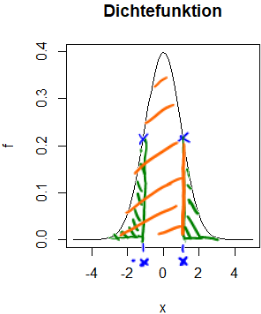
\includegraphics[scale=0.3]{./pic/NormalverteilungDichtefunktion.png}
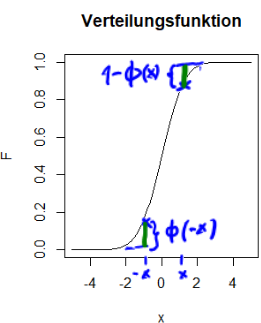
\includegraphics[scale=0.3]{./pic/NormalverteilungVerteilungsfunktion.png}
\textbf{Schätzwerte:}
$ Z = \frac{x-\mu}{\sigma} \thicksim N_ {0,1}$
\subsubsection{Exponentialverteilung}
Modellierung von Lebensdauern, Wartezeiten Sei $ Y_{t} \thicksim P_{\lambda t} $ im Intervall $ [0,t] $  von $ t $  Zeiteinheiten, dann beschreibt die Exponentialverteilung die Wartezeit $ X $ bis zum Eintreten eines Ereignisses; 
\textbf{Dichte- und Verteilungsfunktion:} 
$ f(x) = \lambda e^{-\lambda x} (x \ge 0) $ und 
$ F(x) = 1 - e^{-\lambda x}$; 
\textbf{Verteilung:} 
$ X \thicksim Exp_{\lambda}$; 
$ E[X] = \frac{1}{\lambda} \Rightarrow$ Berechnung mit partieller Integration; 
$ Var[X] = \frac{1}{\lambda^2}$;
\textbf{R:} 
$ \textcolor{red}{d}exp(x,\lambda) = f(x)$; 
$ \textcolor{red}{p}exp(x,\lambda) = F(x)$; 
\textbf{Eigenschaft:} 
Eine exponentialverteile ZV X ist gedächtnislos, d.h. 
$ P(X > s + t) | X > t = P( X > s)$; 
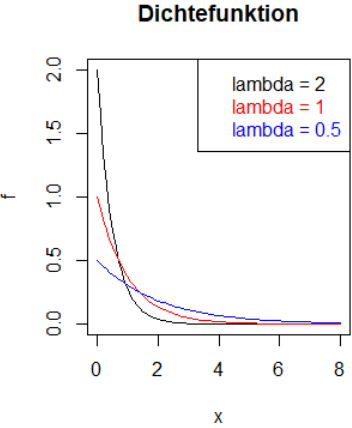
\includegraphics[scale=0.25]{./pic/ExponentialverteilungDichtefunktion.png}
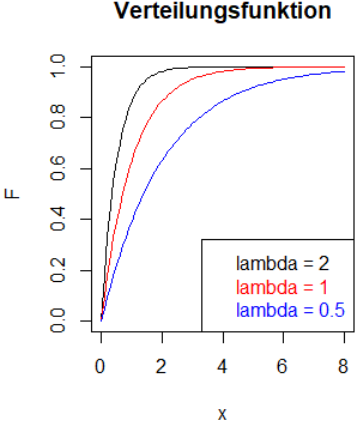
\includegraphics[scale=0.25]{./pic/ExponentialverteilungVerteilungsfunktion.png}
\subsubsection{Chiquadrat-Verteilung}
$ Z_{1},...,Z_{n}$ seien unabhängige, standardnormalverteilte ZV $\Rightarrow  X=Z_{1}^2+···+Z_{n}^2 $ hat Chiquadratverteilung mit n Freiheitsgraden;
\textbf{Anwendungsmodell:} 
Summen unabhängiger, standardnormalverteilter ZV;
\textbf{Verteilung:} 
$ X \thicksim  \chi_{n}^2$; 
$ E[X] = n $; 
$ Var[X] = 2n $; 
\textbf{R:} 
$ \textcolor{red}{d} chisq(x,n)=f(x)$; 
$\textcolor{red}{p} pchisq(x,n)=F(x)$; 
\textbf{Eigenschaft:} 
$ X_{1} \thicksim \chi_{n1}^2 $ und $ X_{2} \thicksim \chi_{2}^2 \Rightarrow X_{1} + X_{2} \thicksim \chi_{n_{1} + n_{2}} $
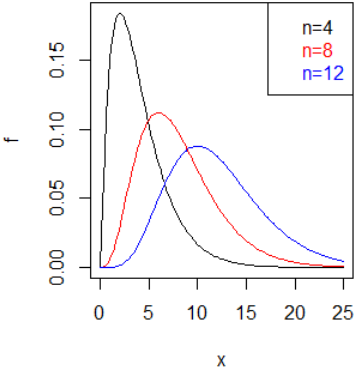
\includegraphics[scale=0.25]{./pic/Chiquadratverteilung.png}
\subsubsection{t-Verteilung}
$ Z \thicksim N_{0,1} $ und $ X \thicksim \chi_{n}^2 \Rightarrow Y = \frac{Z}{\frac{X}{\sqrt{n}}} $ ist t-verteilt mit n Freiheitsgraden; 
\textbf{Anwendungsmodell:}
Schätz- und Testverfahren bei unbekannter Varianz; 
\textbf{Verteilung:} 
$ Y \thicksim t_{n} $; 
$ E[Y] = 0  $ für $ n > 1 $; 
$ Var[Y] = \frac{n}{n-2} $ für $ n > 2 $; 
\textbf{R:} 
$\textcolor{red}{d}t(y,n) \hat{=} f(x) $; 
$ \textcolor{red}{p}t(y,n) \hat{=} F(x)$; 
$ \textcolor{red}{q}t(y, n) \hat{=} F^{-1}(x)$; 
\textbf{Eigenschaften:} 
Für $ n  \rightarrow \infty : t_{n} \rightarrow N_{0,1}$; 
Achsensymmetrie der Dichtefunktion $ \Rightarrow -y_{p} = x_{1-p} $
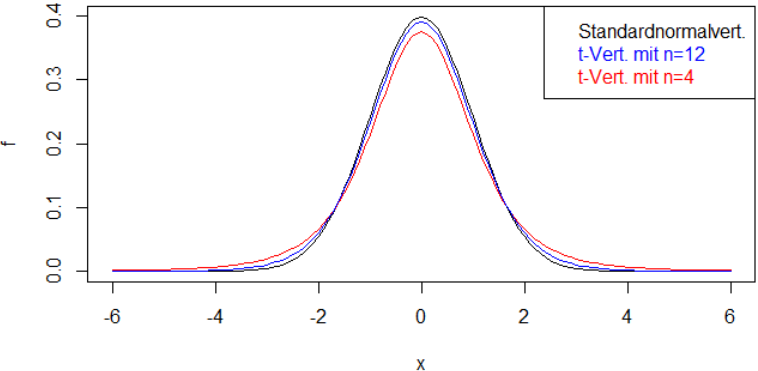
\includegraphics[scale=0.25]{./pic/t-Verteilung.png}\\
Abbildung Dichtefunktion
\section{Zentraler Grenzwertsatz}
$\mu \sigma^2$ bekannt aber nicht die Verteilung
\subsection{ZGWS}
Seien $ X_{i} (i=1, ..., n)$ unabhängige identische verteilte \textbf{(i.i.d)} ZV mit Erwartungswert $\mu$ und Varianz
$ \sigma^2 $. Dann gilt für hinreichend große n ( >30) und $\overline{X} = \frac{1}{n} \sum_{i=1}^{n}$ näherungsweise:\\
$\sum_{i=1}^{n} X_{i}  \thicksim  N_{n\mu, n\sigma^2}$  \&\\
%bezieht sich auf $X_{i}$\\
$\frac{\sum X_{i}-n\mu}{\sqrt{n}\cdot \sigma} \thicksim N_{0,1} $\\
$\sum X_{i} $ bezieht sich auf Y; $\sum X_{i} - n\mu$ bezieht sich auf $ X_{i}$; 
$ \overline{X} \thicksim N_{\mu, \frac{\sigma^2}{n}} $ \& $ \frac{\overline{X}-\mu}{\sigma} \sqrt{n} \thicksim N_{0,1} $; 
Der Satz gilt sogar allgemeiner, wenn die $X_{i}$ abhängig und nicht identisch verteilt sind, vorausgesetzt kein $ X_{i} $ ist deutlich dominanter?! als die anderen.Für die Voraussetzung des  ZGW ist, dass die $ X_{i} $ nicht normalverteilt sein müssen., damit $\sum_{i=1}^{n} X_{i}$ oder $\overline{X}$  bei \textbf{hinreichend großem n} normalverteilt sind. Faustregel: \textbf{Je} schiefer die Verteilung der $ X_{i}$ , \textbf{desto} größer muss n sein: 
\textbf{n>30}: falls die unbekannte Verteilung ohne markanten Ausreißer, aber schief ist (Exponentialverteilung); 
\textbf{n>15:} falls die unbekannte Verteilung annähernd symmetrisch ist(Binomialverteilung); 
$ \boldsymbol{ n \le 15 }$: falls die unbekannte Verteilung annähernd normalverteilt ist; 
\subsection{$\phi$}
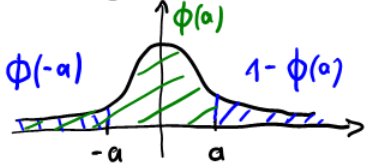
\includegraphics[scale=0.25]{./pic/ZGWPhiVerteilung.png} $ \phi(-a ) = 1 - \phi(a) $; $\phi(a) = 1-\phi(-a) $; 
$ P(-a < Z < a) = \phi(a) - \phi(-a) = \phi(a) - (1-\phi(a)) = \underline{ 2\phi(a) -1 } $ or $ 1-\phi(-a) - \phi(-a) = 1 -2\phi(-a)$
\subsection{$\phi^{-1}$}
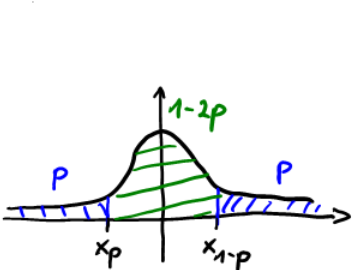
\includegraphics[scale=0.25]{./pic/ZGWPhi-1Verteilung.png}
$  -x_{p} = x_{1-p} \Leftrightarrow -qnorm(p) = qnorm(1-p) \Leftrightarrow -\phi^{-1}(p) = \phi^{-1}(1-p) $
\textbf{Zusammenhang}
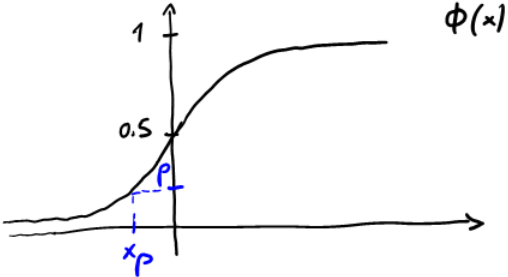
\includegraphics[scale=0.25]{./pic/ZGWSigmoidFunction.png} $ \phi^{-1}(p) = x_{p} $; 
\textbf{Aufgabentypen:} 
Seien $ X_{i} $ i.i.d. ZV mit $\mu$ und $ \sigma^2 $, aber unbekannter Verteilung. Dann sind $ Z_{1} = \frac{\sum X_{i}-n\mu}{\sqrt{n}\sigma}$ und $Z_{2} = \frac{\overline{X}-\mu}{\sigma} $  näherungsweise standardnormalverteilt.\\
	$\circ$ Es lassen sich Wahrscheinlichkeiten für $\sum X_{i}, \overline{X}, Z_{1}$ oder $ Z_{2} $ berechnen.\\
	$\circ$ Es lässt sich \textcolor{red}{n} bestimmen, so dass, zu vorgegebener Schranke $ k $ und Wahrscheinlichkeit $ p $ gilt: $ P(Z_{i} > k) \geq p $ or $ P(-k \leq Z_{i} \leq k) \geq p $
\subsection{Stichprobenvert.normalvert.\\Grundgesamt.}
\subsection{Stichprobenmittel}
Die Stichprobenfunktion $ \overline{X} = \frac{1}{n} \sum_{i=1}^{n} X_{i} $ ist eine erwartungstreue Schätzfunktion für Erwartungswert $ \mu $, d. h.$E[\overline{X}] = \mu$
\subsection{Stichprobenvarianz}
Die Stichprobenfunktion $ S^2 = \frac{1}{n-1} \sum_{i=1}^{n} (X_{i} - \overline{X})^2 = \frac{1}{n-1}(\sum_{i=1}^{n}X_{i}^2 - n\overline{X}^2)$ist eine erwartungstreue Schätzfunktion für die Varianz $\sigma^2$, d. h. $E[S^2] =\sigma^2$; 
$ E[\overline{X}] = E[\frac{1}{n}\sum X_{i}] = \frac{1}{n} E[\sum X_{i}] = \frac{1}{n} \sum_{i=1}^{n} E[X_{i}] = \frac{1}{n} n\mu = \mu$; 
$ Var[\overline{X}] = Var[\frac{1}{n}\sum X_{i}] = \frac{1}{n^2} Var[\sum X_{i}] = \frac{1}{n^2}n\sigma^2 = \frac{\sigma^2}{n} $; 
Seien $ X_{i} (i=1, ..., n)$ unabhängige normalverteilte ZV mit Erwartungswert $\mu$ und Varianz $\sigma^2$. Dann gilt:
\textbf{bei bekannter Varianz:} $ \frac{\overline{X} -\mu}{\sigma} \sqrt{n} \thicksim N_{0,1}$; 
$ \frac{(n-1)S^2 = \sum(x-\overline{x})^2}{\sigma^2 \Rightarrow \text{Standardisierung}} \thicksim \chi_{n-1}^{2}$; 
\textbf{Bei unbekannter Varianz:} $ \frac{\overline{X}-\mu}{S}\sqrt{n} \thicksim t_{n-1}$; 
\section{Konfidenzintervall}
  \subsection{Begriffe}
   Irrtumswahrscheinlichkeit = $ \alpha $; 
  Konfidenzniveau =  $ 1-\alpha $ ; 
  Konfidenzintervall = $ I $
  \subsection{Punkschätzer}
  E[X]: Stichprobenmittel:
  $ \overline{X = \frac{1}{n}} \sum_{i=1}^{n} X_{i}$; 
  Varianz: Stichprobenvarianz:
  $ s^{2} = \frac{1}{n -1} \sum_{i=1}^{n} (X_{i} - \overline{X})^{2} $; 
  Schätzwert für wahren Parameter, aber keine Aussage über Unsicherheit der Schätzung, Geringe Sicherheit für wahren Parameter; 
  
  \subsection{Intervallschätzer}
  Intervall für wahren Parameter, mit vorgegebener Sicherheit; Vorgabe (95\% or 99\%); 
  Dichtefunktion:
  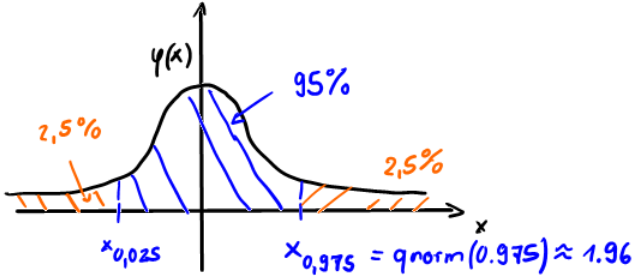
\includegraphics[scale=0.25]{./pic/KonfidenzintervallDichtefunktion.png}
  $ P(-a \le \overline{x} \le a) > 0.95 $; 
  $ \sigma ist $ unbekannter Parameter\\
  $ P( x_{\underbrace{0.025}} < \underbrace{ \frac{\overline{x} - \mu}{\sigma}\sqrt{n} } < x_{\underbrace{0.975}} ) \ge 0.95 $\\
  $ -1.96; N_{0,1}; 1.96 $; 
  
  \subsection{$ \mu $, unbekannt, $ \sigma^{2} $, bekannt}
  $ I = ] \overline{X} \textbf{-} \underbrace{\phi^{-1}( 1-\frac{\alpha}{2} ) } \frac{\sigma}{ \sqrt{n} }\textbf{,} $\\ 
  $ qnorm ( 1-\frac{\alpha}{2} ) $\\
  $ \overline{X} \textbf{+} \phi^{-1} ( 1- \frac{\alpha}{2} ) \frac{\sigma}{ \sqrt{n} } [ $; 
  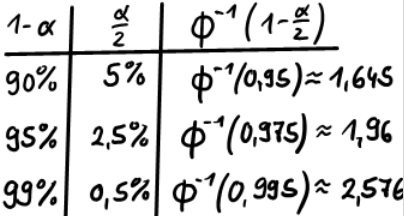
\includegraphics[scale=0.25]{./pic/QnormTabelle.png}
  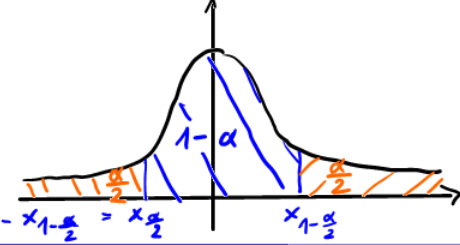
\includegraphics[scale=0.25]{./pic/KonfidenzintervallDichtefunktionTabelle.png}

  \subsection{$ \mu $ \& $ \sigma^{2} $, unbekannt }
  $ I = ] \overline{X} \textbf{-} t_{n-1}^{-1} ( 1-\frac{\alpha}{2} ) \frac{S}{ \sqrt{n} } \textbf{,} \overline{X}  \textbf{+} t_{n-1}^{-1} ( 1-\frac{\alpha}{2} )\frac{S}{ \sqrt{n} } [ $
  \subsection{Zusammenfassung}
  Wie verändert sich das $ (1 - \alpha ) $-Konfidenzintervall, n-größer $\Rightarrow$ I kürzer; 1-$ \alpha $ größer $ \Rightarrow $ I länger; 
  Für $ \frac{L}{2} = 2 \phi^{-1}( 1-\frac{ \alpha}{2} ) \frac{\sigma}{ \sqrt{n} } \frac{1}{2} = 2 \phi^{-1} ( 1- \frac{ \alpha }{2} ) \frac{\sigma}{ \sqrt{4n} } $
  \subsection{Aufgabentypen}
  \textbf{Geg: } n, 1-$ \alpha $; 
  \textbf{Ges: }I s.o.
  \textbf{Geg: }$ \overline{X}, \sigma, 1- \alpha, L $; 
  $ L = 2 \phi^{-1} ( 1-\frac{ \alpha }{2} ) \frac{\sigma}{ \sqrt{n} }$; 
  \textbf{Ges: }n; $ \sqrt{n} > 2\phi^{-1} ( 1- \frac{ \alpha}{2} )\frac{ \sigma }{L} $
  \textbf{Geg: }n, I, L; 
  \textbf{Ges: }1- $\alpha$; 
$ 1- \frac{ \alpha }{2} = \phi (\frac{ L \sqrt{n} }{ 2\sigma} ) $
  
\section{Hypothesentests}
Basierend auf n unabhängig und identisch Verteilte (i.i.d) Zufallsvariablen $ X_{1}, ..., X_{n} $(Messungen) soll eine Entscheidung getroffen werden, ob eine Hypothese für einen unbekannten Erwartungswert $ \mu $ gültig ist or nicht.
\subsection{Def}
$\alpha $ = Signifikanzniveau/ Fehlerwahrscheinlichkeit 
TG = Prüfgröße; 
TG* = standardisierte Prüfgröße; 
siginifikante Schlussfolgerung = $ H_{0} $ verworfen $\rightarrow$ klassischer Parametertest; 
schwache Schlussfolgerung = $ H_{0} $ wird nicht verworfen $\rightarrow$ klassischer Parametertest.
p-Wert = beobachtetes Signifikanzniveau
\subsection{Null- und Gegenhypothese}
\textbf{Modell:} Verteilung der Grundgesamtheit or Testgröße \textbf{TG} ( häufig $\overline{x}$ ) ist bekannt bis auf einen Parameter, z.B. $ \mu $, für den eine Hypothese aufgestellt wird.
$ TG \sim  N_{\mu, \sigma^2}$; 
\textbf{Nullhypothese: $ H_{0}$:} Angezweifelte Aussage, der widersprochen werden kann, wenn die Stichprobe einen Gegenbeweis liefert. $ H_{0}: \mu = \mu_{0}$; 
\textbf{Gegenhypothese $ H_{1} $:} Gegenteil von $ H_{0} $ z.B. $ H_{1} \neq \mu_{0} $;
\subsection{Ablehnungsbereich, Fehler 1. \& 2.}
Treffen der Testentscheidung, basierend auf einer konkreten Stichprobe 
$ \{x_{1}, ..., x_{n} \} $; Berechnung der Realisation $ tg = TG(x_{1},..., _x{n}) $ der Prüfgröße TG; 
\textbf{Ablehnungsbereich / Kritischer Bereich C}: Werte der Testgröße, die für H1, sprechen \& bei Gültigkeit von $ H_{0} $ mit Wahrscheinlichkeit $ \le \alpha $ ( meist 0.1, 0.05, or 0.01) auftreten.\textbf{Fehler 1. Art:}$ \alpha $ ist die Wahrscheinlichkeit, dass $ H_{0} $ verworfen wird, obwohl sie richtig ist.
\textbf{Annahmebereich:} Komplement $ \overline{C} $ des Ablehnungsbereichs. $ H_{0} $ kann nicht abgeleht werden, falls $ tg \in \overline{C} (P(tg \in \overline{C}) \ge 1 - \alpha) $.\textbf{Fehler 2. Art:} Die Wahrscheinlichkeit, dass $ H_{0} $ nicht abgelehnt wird, obwohl sie falsch ist.
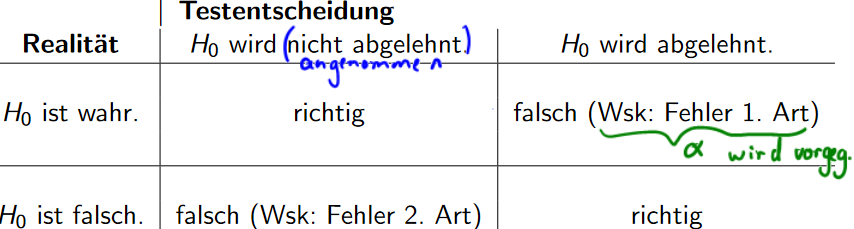
\includegraphics[scale=0.25]{./pic/Testzenarien.png}
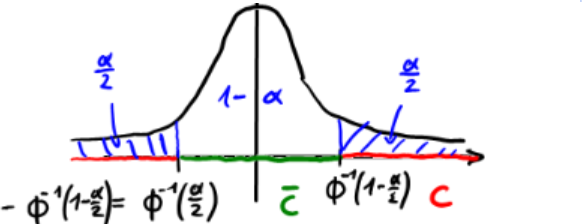
\includegraphics[scale=0.25]{./pic/StandardnormvalverteilungTestgroese.png}
$H_{0}: \mu = \mu_{0} $; $ H_{1}: \mu \neq \mu_{0} $; 
\subsection{Klassischer Parametertest}
$H_{0} $ wird abgelehnt, falls $ tg = TG( x_{1}, ..., x_{n} ) \in C $; 
$ H_{0} $ wird angenommen falls $ tg = TG(x_{1}, ..., x_{n}) \in \overline{C} $; 
Der kritische Bereich ergibt sich analog zu den Konfidenzintervallen durch die Vorgabe eines kleinen Signifikanzniveau $ \alpha $ d.h. max. Wahrscheinlichkeit für Fehler 1. Art, mit standardisierter Prüfgröße TG* gilt:
$ P (TG \in C) \le \alpha  \Leftrightarrow TG^{*} \in ]-\infty; \phi^{-1}(1- \frac{\alpha}{2}) [ \cup ] \phi^{-1}(1-\frac{\alpha}{2}); \infty [$; 
$ P(TG \in \overline{C}) \ge 1 - \alpha \Leftrightarrow TG^{*} \in [ \phi^{-1}(\frac{\alpha}{2}), \phi^{-1}(1-\frac{\alpha}{2}) ] $; 
Wird dann $ H_{0} $ verworfen, spricht man von einer signifikanten Schlussfolgerung. Kann $ H_{0} $ nicht verworfen werden, dann lässt sich keine Aussage über den Fehler 2. Art treffen \& man spricht von einer schwachen Schlussfolgerung.
\subsection{Zweiseitiger Gauß Test}
$ H_{0}: \mu = \mu_{0}  $ gegen $ H_{1}: \mu \neq \mu_{0} $; 
$ \overline{ X } \sim  N_{ \mu_{0}, \sigma_{0}^2 /n} \Rightarrow \frac{ \overline{X} - \mu_{0} }{ \sigma_{0} } \sqrt{n} \sim N_{0, 1} $; 
$ P_{ \mu0}( \overline{X} \in C ) \le \alpha \Leftrightarrow |TG| = \frac{ | \overline{X} - \mu_{0} | }{ \sigma_{0} } \sqrt{n} > \phi^{-1}(1-\frac{ \alpha}{2} )$; 
\textbf{Testentscheidung:} $ H_{0} $ wird abgelehnt, falls $ |TG| > \phi^{-1}(1-\frac{ \alpha }{ 2 } ) $; $ H_{0} $ wird angenommen, falls $ |TG| \le \phi^{-1}(1-\frac{ \alpha }{2} )$
\subsection{Einseitiger Gauß Test}
\subsubsection{linksseitig}
$ H_{0}: \mu \ge \mu_{0} $ gegen $ H_{1}: \mu  < \mu_{0}$
\subsubsection{rechtsseitig}
$ H_{0}: \mu \le \mu_{0} $ gegen $ H_{1}: \mu > \mu_{0} $
\hrule
$ P_{\mu 0} ( \overline{X} \in C ) \le \alpha \Leftrightarrow TG = \frac{ \overline{ X } - \mu_{0} }{ \sigma_{0} } \sqrt{n} < \phi^{-1} ( \alpha ) $; 
\textbf{Testentscheidung:} $ H_{0} $ wird abgelehnt falls, $ TG < \phi^{-1} ( \alpha )$; 
$ H_{0} $ wird angenommen, falls $ TG \ge \phi^{-1} ( \alpha ) $; 
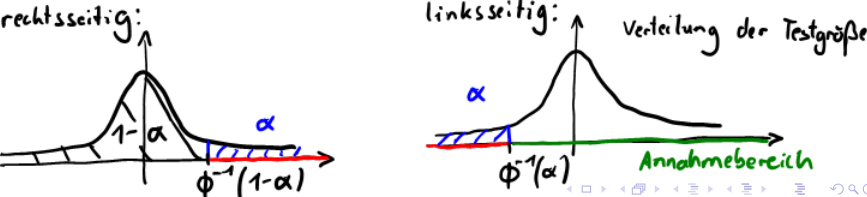
\includegraphics[scale=0.25]{./pic/EinseitigerGausTest.png}
\subsection{Varianten Gauß Test, $ \sigma^2 $ bekannt, $\mu$ unbekannt}
Prüfgröße$ tg = \frac{ \overline{X} - \mu_{0} }{ \sigma_{0} }\sqrt{n} $; \\
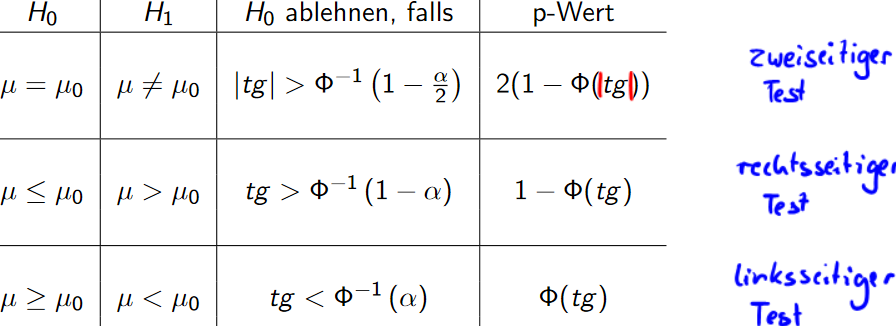
\includegraphics[scale=0.25]{./pic/GausTests.png}
\subsection{t-Test, $ \mu, \sigma^2 unbekannt  $}
Prüfgröße $ tg = \frac{ \overline{X} -\mu_{0} }{ S } \sqrt{n} \sim t_{n-1} $
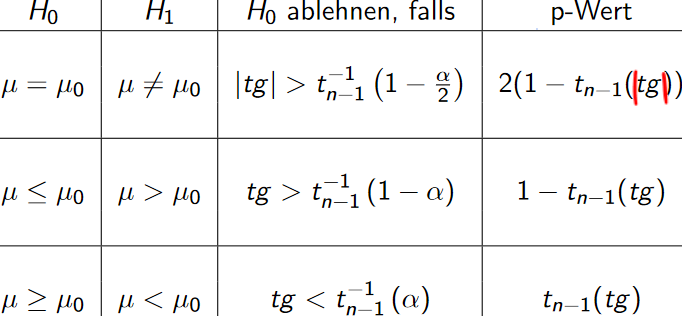
\includegraphics[scale=0.25]{./pic/tTest.png}
\subsection{p-Wert}
Wahrscheinlichkeit, bei Zutreffen von $ H_{0} $ den beobachteten Wert tg der Prüfgröße or einen noch stärker von $ \mu_{0} $ abweichenden Wert zu bekommen.
%Grafik p-Value slide 15+1?
Der p-Wert zu einer Hypothese $ H_{0} $ ist der kleinste Wert von $ \alpha $, für den $ H_{0} $ noch abgelehnt werden kann. \textbf{Je kleiner} der Wert, \textbf{desto kleiner} ist der Fehler 1. Art \& umso signifikanter ist die Testentscheidung. 
\textbf{Nice to know} Anhand des p-Werts kann man für beliebige Werte von $ \alpha $ eine Testentscheidung treffen;\\
Falls $ p-Wert < 1\%:$ sehr hohe Signifikanz\\
Falls $ 1\% \le p-Wert < 5\%: $ hohe Signifikanz\\
Falls $ 5\% \le p-Wert \le 10\%: $ Signifikanz\\
Falls $ p-Wert > 10\%: $ keine Signifikanz\\
\subsection{Zusammenhang I \& Hypothesentests zweiseitig}
zum Konfidenzniveau $ 1- \alpha $; 
$ H_{0} $ wird abgelehnt, falls $ \mu_{0} \notin I $; 
$ H_{0} $ wird angenommen, falls $ \mu_{0} \in I $; 
Das Konfidenzniveau ist der Annahmebereich von $ H_{0} $ zum Signifikanzniveau $ \alpha $; 
\subsection{Zusammenfassung klass. Hypo.test}
Signifikanzniveau $ \alpha $ wird vorgegeben;\\
$ \alpha $ \& Verteilung der Testgröße unter $ H_{0} $ wir der Ablehnungsbereich ermittelt. \textbf{Je kleiner (größer) } $ \alpha $ , \textbf{desto kleiner (größter) } ist der Ablehnungsbereich; \\
\textbf{!:} $ \alpha \& C $  hängen \textbf{nicht von} der konkreten Stichprobe ab;\\
$ H_{0} $ wird abgelehnt, falls der ermittelte Wert der Testgröße (beobachteter Wert) in C liegt. 
\textbf{!:} Die tg hängt von der konkreten Stichprobe ab. Sie ist eine ZV.
\subsection{Test mittels p-Wert}
$ \alpha $ wird vorgegeben.\\
Berechnung des p-Werts anhand der konkreten Stichprobe mit der Verteilung der Tg unter $ H_{0}  $;\\
\textbf{!:}Der p-Wert hängt von der konkreten Stichprobe ab, ist eine ZV.\\
$ H_{0} $ wird abgelehnt, falls $ p-Wert \le \alpha. $;


\section{Fehleranalyse}
\subsection{Auslöschung}
wenn ungefähr gleich große, bereits mit Fehlern behaftete Zahlen voneinander abgezogen werden \& signifikante Mantissenstellen ausgelöscht werden.
\subsection{Addition}
große signifikante Stellen schlucken kleine signifikante Stellen.
\subsection{Horner}
Ohne: Runden bei jeder Rechenoperation. Mit: Vermeidung der Rundungsfehler nach jeder Rechenoperation.
\subsection{Abc-Formel}
$ x_{1,2} = \frac{-b \pm \sqrt{b^2 - 4ac}}{2a} $; 
$ x_{1,2} = \frac{2a}{-b \mp \sqrt{b^2 -4ac}} $; 
b>0, dann (2), für $ x_1 $ \&(1) für $ x_2 $ or 
b<0, (1) für $x_{1} $ \& (2) für $ x_2 $;
Falls 4ac klein im Vergleich zu $ b^2$, dann evtl. Probleme der Auslöschung.
\subsection{Stabilität}
Verfahren, wenn es gegenüber kleinen Störungen unempfindlich ist. Rundungsfehler nicht zu stark auf die Berechnung auswirken. Man unterscheidet bei der numerischen Lösung mathematischer Probleme Kondition, Stabilität und Konsistenz. Stabilität ist dabei eine Eigenschaft des Algorithmus und die Kondition eine Eigenschaft des Problems. Die Beziehung zwischen diesen Größen lässt sich wie folgt beschreiben:
$f(x) $ =mathematische Problem in Abhängigkeit von der Eingabe $ x, \tilde{f}$ = numerische Algorithmus, 
$ \tilde{x} $ = gestörten Eingabedaten:
$ || f(\tilde{x}) - f(x) || $ Kondition: Schwankung des Problems bei Störung; 
$ ||\tilde{f}( \tilde{x} ) - \tilde{f} (x) || $ Stabilität: Schwankung des numerische Algorithmus bei Störung; 
$ ||\tilde{f}(x)-f(x) || $ Konsistenz: Wie gut löst der Algorithmus (mit exakter Eingabe) tatsächlich das Problem; 
$ || \tilde{f}( \tilde{x} )-f(x)|| $Konvergenz: Wie gut löst der gestörte Algorithmus das Problem; 
\section{Interpolation}
Zu gegebenen Punkten $ ( x_{i}, y_{i} ), i=0, ..., n $ mit $ x_{i} \neq x_{j} $ für $ i \neq  j $ eine Funktion G ( dies ist nicht eindeutig! Abhängig von der Funktionsklasse ), so dass $ G ( x_{i} ) = y_{i}, i=0, ..., n $ (Interpolationsbedingung). Interpolation ist \textbf{ungeeignet} für verauschte Daten. Lösung: Approximation der kleinsten Quadrate.

\subsection{Begriffe}
Extrapolation $\hat{=} $ Näherungwerte für x-Werte außerhalb der Stützstellen;\\
Dividierende Differenzen $\hat{=}$ Koeffizienten $ c_{i} $ lassen sich rekursiv durch wiederholte Bildung von "Differenzquotienten" berechnen
\subsection{Vandermonde/klassisch}
Unterschiedliche Darstellungen für ein Interpolationspolynom $ G(x) = p_{n}(x) $ vom Grad $ n $ haben unterschiedliche Eigenschaften bei der numerischen Berechnung.\textbf{Monombasis:} $ x^{0}, x^{1}, x^{2}, x^{3}, ...; p_{n}(x) = a_{n} x^n + ... + a_{1} x^{1} + a_{0} x^{0} $; 
\textbf{Ziel:} Bestimmung d. Koeffizienten $ a_{0}, a_{1}, ..., a_{n} $ sodass $ p_{n}( x_{i} ) = y_{i} = a_{n} x_{i}^n + ... + a_{1} x_{i}^1 +a_{0} x^{0} $ für i = 0, ..., n; 
\textbf{Für die eindeutige Lösung n+1 Gleichungen: Interpolationsbedingungen};
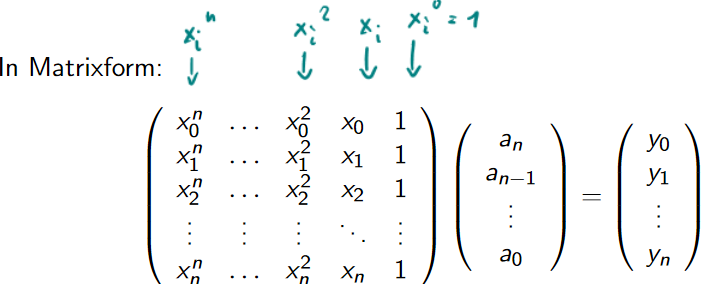
\includegraphics[scale=0.25]{./pic/VandermondeMatrix.png}
Die Koeffizientenmatrix ist die sog. \textbf{Vandermonde Matrix}; \textbf{Eigenschaften:} Die Vandermonde Matrix ist nicht singulär( falls alle $ x_{i} $ verschieden); Rechenaufwand: $ \mathcal O ( n^{3} ) $; Für große n sehr schlecht konditioniert \& als Allgemeiner Ansatz ungeeignet.

\subsection{Lagrange}
\textbf{2 Formeln}; 
$ p_{n}(x) = y_{0} L_{0} (x) + y_{1} L_{1} (x)+ ... +y_{n} L_{n} (x) $;
$ L_{k}(x) \prod_{ j = 0;j\neq k }^{n} \frac{ x-x_{j} }{ x_{k} - y_{j} } $; 
Jede Basisfunktion $ L_{k}(x) $ ist ein Polynom vom Grad $ \le n $; 
\textbf{Bemerkung:} Findet Anwendung bei Numerischer Integration; Wenn Stützstellen $ x_{i}  $ gleich bleiben \& nur $ y_{i} $ ändern $ \Rightarrow $ keine Neuberechnung; Rechenaufwand $ \mathcal O ( ( n +1)^{2} ) $; Kommen neue Stützpunkte hinzu $ \Rightarrow $ Neuberechnung\textbf{!}; Die Interpolationspolynome liefern nur sinnvolle \textbf{ Näherungswerte } für x-Werte, die zwischen den gegebenen Stützstellen liegen; Extrapolation ( Näherungwerte für x-Werte außerhalb der Stützstellen ) kann zu großen Abweichungen führen.

\subsection{Newton}
Darstellung des Interpolanten, die auf ein gestaffeltes LGS führt \& einfache Hinzunahme weiterer Punkte erlaubt.
$p_{n}(x) = c_{0} + c_{1} ( x-x_{0} ) + ... + \underbrace {c_{n} ( x-x_{0} ) ( x-x_{1} ) ... ( x-x_{n-1} ) } $\\
Polynom vom Grad n\\
Das Resultierende LGS für die Koeffizienten $ c_{i} $ hat gestaffelte Form.
\textbf{Interpolationsbedingungen?}\\
\textbf{Vorteile:} Rechenaufwand $ \mathcal O ( n^{2} ) $ Gleitpunktoperationen; Hinzufügen weiterer Stützstellen ohne großen Aufwand. Andere Koeffizienten bleiben unverändert.

\subsection{Dividierende Differenzen}
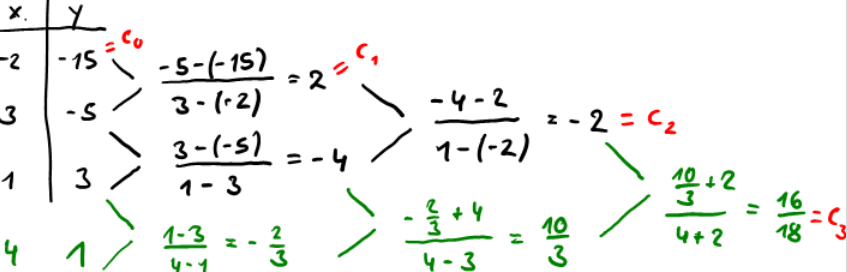
\includegraphics[scale=0.25]{./pic/DividierendeDifferenzen.png}

\subsection{Effizienz}
\subsection{klasisch}
$ p_{n} (x) = a_{n} x^{n} + ... + a_{0} $; 
\textbf{Aufwand:} 2n-1 Mult.
\subsection{Horner Schema}
$ p_{3} (x) = a_{3} x^{3} + a_{2} x^{2} + a_{1} + a_{0} = (( a_{3} + a_{2} ) x + a_{1} )x+ a_{0} $; 
Allg.: $ p_{n} (x) = ( ... ( a_{n} x + a_{n-1} ) x + ... + a_{1} ) x + a_{0} $; 
\textbf{Aufwand:} n Mult.

\subsection{Interpolationsfehler}
Falls $ f $ hinreichend glatt ist \& $ p_{n} $ das eindeutige Interpolationspolynom von Gradn $ n $, dann gilt fürn den Interpolationsfehler:
$ f(x) - p_{n}(x) = \underbrace{ \frac{ f^{ ( n+1 ) }( \theta ) }{ ( n+1) ! } ( x-x_{0} )...( x-x_{n} ) } $ mit $ \theta \in [ x_{0}; x_{n} ]  $\\
Vergleichbar zum Restglied bei der Taylorreihenentwicklung; 
\textbf{Bemerkung:} $ \theta $ unbekannt, daher nur Fehlerabschätzung; 
Fehler ist Abhängig von der Verteilung der Stützstellen; 
Der Fehler ist bei großen n an den Intervallrändern deutlich größer, als in der Intervallmitte
\subsection{Wahl der Stüztstellen}
Runge Funktion $ (f) = \frac{ 1 }{ 1+25x^{2} } $ äquidistante Stützstellen das Interpolationspolynom nicht immer gegen die zugrundeliegende stetige Funktion konvergiert, wenn die Anzahl der Stützstellen \& damit der Grad des Polynoms wächst.\textbf{Lösung:}  Nicht-aquidistante Verteilung der Stützstellen, dichter an den Intervallgrenzen.
\subsection{Chebyshev-Punkte}
haben die Eigenschaft; senkrechte Projektion von gleichverteilten Punkten auf dem Einheitskreis. $ t_{k} = cos\frac{ ( 2k-1 ) \pi }{ 2n }, k=1,...,n, auf ]-1,1[ $;  Invtervall: $ ]a,b[: x_{k} = \frac{ a +b }{2} + \frac{ b-a }{ 2 } t_{k} $. $\Rightarrow$ Fehler wird gleichmäßiger verteiltund Konvergenz erreicht.
\subsection{Schwächen der Polynominterpolation}
Hoher Rechenaufwand bei meist keiner hoher Differenzierbarkeitsgrad benötigt wird; RB kann Interpolationsfehler sehr groß sein; Bei wachsenden $n$ ist es unmöglich eine Konvergenz gegen die zu interpolierenden Funktion sicherzustellen;
\textbf{R:} 
approx $\hat{=}$ lin Interpolation; 
Spline $\hat{=}$ Spline interpolation; 
Bibliotheken für Polynominterpolation;
\subsection{Spline}
%Hinreichend glatte (( k -1 ) - mal stetig differenzierbare ) \& abschnittsweise aus Polynomen zusammengesetzte Funktion $ \hat{ = } $ Splines vom Grad $ k $ ( meist k = 2 or k =3 ).
Jede Funktion $ S_{i} $ ist ein Polynom vom Grad  $ n \le k $ ; 
$ S(x) $ ist $ ( k -1 ) $ - mal stetig differenzierbar, d.h. für alle $ x_{i} ( i = 1, ..., n-1 ) $ gilt: $ S_{ i-1 } ( x_{ i } ) = S_{ i } ( x_{i} ) $; 
\subsection{Kubisch}
\textbf{Ansatz:} $ S_{ i } = a_{ i } + b_{ i } ( x- x_{ i } ) + c_{ i } (x-x_{i})^{2} + d_{i} (x-x_{i})^{3}$; 
\textbf{Gleichungssystem:} 4n Parameter $ a_{i}, b_{i}, c_{i}, d_{i} ( i=0, ..., n-1) $; 
\textbf{2n Interpolationsbedingungen:} am Rand je nur eine. $ S_{i} x_{i} = y_{i}$; 
$ Si (x_{i+1}) = y_{i+1}$ für $  ( i= 0, 1, ..., n-1) \Rightarrow $ Stetigkeit; 
\textbf{Stetigkeit der 1. Abl:} 
$ S_{i}^{'} (x_{i+1}) = S_{i+1}^{'}(x_{i+1}) $; 
$ \Leftrightarrow S_{i}^{'}(x_{i+1}) - S_{i+1}^{'} ( x_{i+1}) = 0 $; 
für $ i = 0, 1, ..., n-2 $; 
\textbf{Stetigkeit der 2. Abl.:} 
$ S_{i}^{''} (x_{i+1}) = S_{i+1}^{''} (x_{i+1}) $; 
$ S_{i}^{''}(x_{i+1}) - S_{i+1}^{''}(x_{i}+1) = 0 $ ; für $ i=0,1,...,n-2) $; 
\textbf{natürlicher Randbedingungen:}
$ S_{0}^{''}(x_{0}) = 0 $; 
$ S_{n-1}^{''}(x_{n}) = 0 $; 
nach geschickter Umformung der Gleichungen hat das LGS Tridiagonalform. 
\textbf{Rechenaufwand} $ \mathcal O ( n ) $ Gleitpunktoperationen.
\section{NumInt}
Verbesserung der Näherung: Aufteilung in kleine Teilintervalle \& Summe von Rechtecksflächen bilden; Interpolations mit Polynom höheren Gredes durch diskrete Punkte.
\subsection{Def}
$ p_{k} \hat{=} $ Interpolationspolynom

\subsection{Newton-Cotes}
Das Intergral des $ p_{k} $ diens al Appr. für das Int. von f(x); 
$ \int_{0}^{1} f(t) dt \approx \int_{0}^{1} p_{k} (t) dt =  \sum_{j=0}^{k} \alpha_j f( t_{j} ) $ Das Interpolationspolynom muss nicht explizit aufgestellt werden, es dient vorab der Bestimmung der Gewichte $ \alpha_{j} $; 
$ \int_{0}^{1} p_{k}(t) = \int_{0}^{1} \sum f( t_{j} ) L_{j} (t) dt = \sum f ( t_{j} ) \int_{0}^{1} L_{j} (t) dt $
\subsubsection{Trapezregel}
$ T_{1}: $ 
$ \int_{0}^{1} f (t) dt \approx \frac{1}{2} ( f(0) + f(1) ) $; 
$ \int_{a}^{b} f (x) dx \approx \frac{(b-a)}{2} (f(a) + f(b) ) $;\\
$ T_{n}: $
Für Teilintervalle mit gleicher Länge: $ h = \frac{b-a}{n} $;  
$ T_{n} = h (\frac{ f ( x_{0} ) }{2} + f(x_{1}) + ... + f(x_{n-1}) + \frac{ f(x_n) }{2} ) $; 
\subsubsection{SimpsonRegel}
$ S_{1}: $ 
$ \int_{0}^{1} f (t) dt \approx \frac{1}{6} ( f(0) + 4f(0.5) + f(1) ) $; 
$\int_{a}^{b} f (x) dx \approx \frac{b-a}{6} ( f(a) + 4f( \frac{a+b}{2}) + f(b) ) $; 
Für n = 1: $\frac{( b-a )}{2\cdot1} \frac{1}{3} ( f(a) + 4f( \frac{a+b}{2}) + f(b) ) $; 
Für n allg.: $ \frac{( b-a) }{2n}\frac{1}{3} ( f(a) + 4(a+h) + ... + 4f(b-h)+ f(b) ) $ 
$ S_{n}:$ 
\textbf{Beachte gerade Anzahl an Teilinvervallen!}; 
Für 2n Teilintervalle, 2n+1 Knoten mit gleicher Länge $ h = \frac{ b-a }{2n} $; 
$ S_{2} = \frac{h}{3} ( f(x_{0}) + 4f(x_{1}) + 2f(x_{2}) + 4f(x_{3}) + f(x_{4}) ) $; 
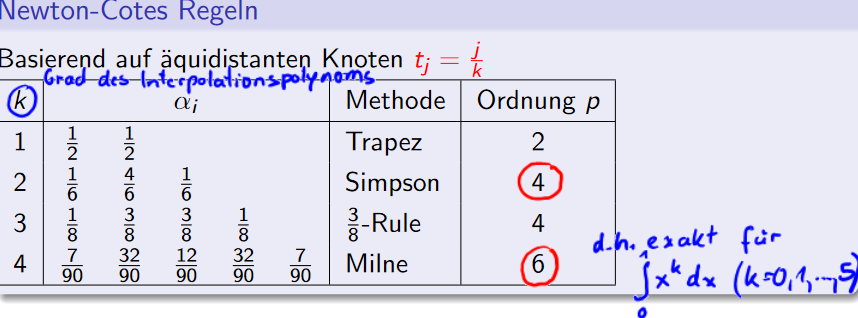
\includegraphics[scale=0.25]{./pic/NewtonCodesRegeln.png}
Falls $\alpha_{i} $ positiv. Integrationsregeln stabil; 
$ k \le 7 \& k =9 \Rightarrow $ positive Gewichte;
Bei halbierung der Intervalle \textbf{Nachfrage} vervierfacht or versechszehnfacht sich der Fehler?
\subsection{FehlerQuadratur}

\section{Allgemein}
\subsection{Symbole}
Stichprobenstandardabweichung $ \hat{=} $ s;
Standardabweichung $ \hat{=} \sigma $
\subsection{Abl.}
$ x^n  \hat{=} nx^{n-1}$
\hrule
$ sin x \hat{=} cos x $; 
$ cos x  \hat{=} - sin x $; 
$ tan x \hat{=} \frac{1}{cos^2 x} = 1 + tan^2 x $;
$ cot x \hat{=} - \frac{1}{sin^2 x} = - 1 -cot^2 x $; 
\hrule
$ e^x \hat{=} e^x $; 
$ a^x \hat{=} (\ln a) \cdot a^x $; 
\hrule
$ \ln x \hat{=} \frac{1}{x} $;
$ \log_a x  \hat{=} \frac{1}{(\ln a) \cdot x}$; 
\hrule
\subsection{Abl.Regeln}
\textbf{Faktorregel} $ y = C \cdot f(x) \Rightarrow  y' = C \cdot f'(x) $; 
\textbf{Summenregel} $ y = f_{1}(x) + f_{2}(x) + ... +f_{n}(x) \Rightarrow y' = f'_{1}(x) + f'_{2}(x) + ... + f'_{n}(x) $; 
\textbf{Produktregel} $ y = u \cdot v \Rightarrow y' = u'\cdot v + v' \cdot u $; 
$ y = u \cdot v \cdot x \Rightarrow y' = u' \cdot v \cdot w + u \cdot v' \cdot w + u \cdot v \cdot x'$; 
\textbf{Quotientenregel} $ y = \frac{u}{v} \Rightarrow y' = \frac{u' \cdot v - u \cdot v'}{v^2}$; 
\textbf{Kettenregel} $ f'(x) = F'(u) u'(x) \hat{=} F'(u): \text{Ableitung der Äußeren Funktion}; u'(x): \text{Ableitung der Inneren Funktion}$
\subsection{Integralregel, elementar}
\textbf{Faktorregel}$\int_{a}^{b}  C \cdot f(x) dx = C \cdot \int_{a}^{b} f(x)dx$; 
\textbf{Summenregel} $ \int_{a}^{b} [f_{1}(x) + ... + f_{n}(x)] dx = \int_{a}^{b} f_{1}(x) dx + ... + \int_{a}^{b}f_{n}(x) dx$; 
\textbf{Vertauschungsregel}$ \int_{b}^{a}f(x) dx = -\int_{a}^{b} f(x) dx$; 
$ \int_{a}^{a} f(x) dx = 0 $; 
$ \int_{a}^{b}f(x) dx = \int_{a}^{c} f(x) dx + \int_{c}^{b} f(x) dx  \text{ für } (a \le c \le b) $; 
\subsection{Berechnung best. Integr.}
$ \int_{a}^{b} f (x) dx = [F(x)]_{a}^{b} = F(b)- F(a) $

\subsection{Bin.Formel}
$ (a + b)^2 = a^2 + 2ab + b^2 $ 1. Binom;
$ (a+b)^3 = a^3 + 3a^2b + 3ab^2 + b^3 $; 
$ (a+b)^4 = a^4 + 4a^3b + 6a^2b^2 + 4ab^3 + b^4$
\hrule
$ (a-b)^2 = a^2 - 2ab + b^2 $; 2. Binom;
$ (a-b)^3 = a^3 - 3a^2b + 3ab^2 - b^3$; 
$ (a-b)^4 = a^4 - 4a^3b + 6a^2b^2 - 4ab^3 + b^4 $
\hrule
$ (a+b) (a-b) = a^2 - b^2 $ 3. Binom; 

\subsection{Wurzel}
$ \sqrt{a ^2} = |a| $;
$ b = a^n  \Leftrightarrow a = \sqrt[n]{b}$; 
$ \sqrt[n]{a} = a^{\frac{1}{n}} $; \\
$ \sqrt[n]{a \pm b} \ne \sqrt[n]{a} \pm \sqrt[n]{b} $ \\
\hrule
$ \sqrt[n]{a^m} = (a^m)^{\frac{1}{n}} = a^{\frac{m}{n}} = (a^\frac{1}{n})^m = (\sqrt[n]{a})^m $ \\
$\sqrt[m]{\sqrt[n]{a}} = \sqrt[m]{a^{\frac{1}{n}}} = (a^{\frac{1}{n}})^{\frac{1}{m}} = a^{\frac{1}{m \cdot n}} = \sqrt[m \cdot n ]{a} $\\
$ \sqrt[n]{a} \cdot \sqrt[n]{b} = (a^{\frac{1}{n}}) \cdot (b^{\frac{1}{n}})  = (ab)^{\frac{1}{n}} = \sqrt[n]{ab} $\\
$ \frac{\sqrt[n]{a}}{\sqrt[n]{b}} = \frac{a^{\frac{1}{n}}}{b^{\frac{1}{n}}} = (\frac{a}{b})^{\frac{1}{n}} = \sqrt[n]{\frac{a}{b}} \text{ für } b > 0 $\\
$\Rightarrow m , n \in \mathbb{N}^*; a \ge  0, b \ge 0 $

\subsection{Potenzen}
$ x^{-n} = \frac{1}{^n} $; 
$ a^0 = 1, a^{-n} = \frac{1}{a^n} $; 
$ a^m \cdot a^n  = a^{m+n} $; 
$ \frac{a^m}{a^n} = a^{m-n} $ für $ a \ne 0 $; 
$ ! (a^m)^n = (a^n)^m = a^{m \cdot n} $; 
$ a^n \cdot b^n = (a \cdot b)^n $; 
$ \frac{a^n}{b^n} = (\frac{a}{b})^n \text{ für } b \ne  0 $; 
$ a >0 : a^b = e^{b \ln a} $; 
$ 0^0 = 1 $; 
$ x_{1}^1 = x_{1} $; 

\subsection{Einigungen}
	$\circ$ Beim Runden mind. eine Nachkommastelle.
\subsection{Trigonometrischer Pythagoras}
$ \sin^2 x + cos^2 x = 1 $
\subsection{e}
$ y = a^{x} = e^{\lambda x} (\lambda = ln a) $; 
Def.Ber.: $ \infty < x < \infty $; 
Wert.ber.: $ 0 < y < \infty$; 
Mon.: $ \lambda > 0 $ d.h. a > 1: str. mon. wachs; $ \lambda < 0 $ d.h. 0 < a > 1): str. mon. fall.; 
Asymp.: y = 0 (x-Achse); 
$ y(0) = 1 $ (alle Kurven schneide die y-Achse bei y = 1); 
$ y = a^{-1} $ entsteht durch Spiegelung von $ y = a^{x} $ an der y-Achse.
\subsection{Logarithm.}
$ y = \log_a x $ mit x>0 ist Umkehrfunktion von $ y = a^{x} $; 
Def.Ber.: x >0; 
Wert.Ber.: $ -\infty  < y < \infty $; 
Nullst.: $ x_{1} = 1 $; 
Monot.: 0 < a < 1: str.mon. fall; 
a > 1; str.mon.wachs.; 
Asymp.: x = 0(yAchse); 
$ log_{a} 1 = 0, log_{a} a = 1 $; 
$ y = log_{a} x $ ist Spieg. von $ y = a^{x} $ an Wink.halb. d. 1. Quadr.

%\input{inhalt/aussagen}
%\input{inhalt/mengen}
%\input{inhalt/relationen}
%\input{inhalt/abbildungen}
%\input{inhalt/beweise} 
%\input{inhalt/graphen}
%\input{inhalt/graphalgo}
%\input{inhalt/bool}
%\input{inhalt/formeln}
\end{multicols*}
\end{document}